% Homework Template
\documentclass[a4paper]{article}
\usepackage{ctex}
\usepackage{amsmath, amssymb, amsthm}
\usepackage{moreenum}
\usepackage{mathtools}
\usepackage{url}
\usepackage{bm}
\usepackage{enumitem}
\usepackage{graphicx}
\usepackage{subcaption}
\usepackage{booktabs} % toprule
\usepackage[mathcal]{eucal}
\usepackage[thehwcnt = 4]{iidef}

\thecourseinstitute{清华大学电子工程系}
\thecoursename{\textbf{媒体与认知} \space 课堂2}
\theterm{2021-2022学年春季学期}
\hwname{作业}
\begin{document}
\courseheader
\name{李智毅}
\vspace{3mm}
\centerline{\textbf{\Large{理论部分}}}

\section{单选题(15分)}
\subsection{\underline{D}}

\subsection{\underline{C}}

\subsection{\underline{B}}

\subsection{\underline{A}}

\subsection{\underline{D}}

\section{计算题(15 分)}



\subsection{假设邮件粗略分为垃圾邮件和正常邮件,且存在一种垃圾邮件的检测方法,其中垃圾邮件被正确检测的概率为a,正常邮件被误判为垃圾邮件的概率为b。针对某一邮箱,所有邮件中垃圾邮件占的比例为c,如果某封邮件被判定为垃圾邮件,根据贝叶斯定理,这封邮件是垃圾邮件的概率是多少?\newline(提示:全概率公式$P(Y)=\sum^{N}_{i=1}P(Y|X_i)P(X_i)$)}
设为垃圾邮件事件为$ A $,不是垃圾邮件的事件为$ \overline{A} $;被判定为垃圾邮件的事件为$ B $,被判定不为垃圾邮件的事件为$ \overline{B} $,则
$$ P(B|A) = a, P(B|\overline{A}) = b, P(A) = c $$
因此,由贝叶斯定理
$$ P(A|B) = \frac{P(A)P(B|A)}{P(A)P(B|A) + P(\overline{A})P(B|\overline{A})} = \frac{ac}{ac + (1-a)b} $$

\subsection{给定样本集合, 其均值为$\mu=[1, 2]^T$, 样本协方差矩阵为$C$,且已知$CU=U\lambda$。\newline 其中$U=\left[ \begin{array}{cc}
    0.5 & -0.4 \\
    0.5 & 0.4
\end{array} \right]$, $\lambda=\left[ \begin{array}{cc}
    10.7 & 0 \\
    0 & 0.4
\end{array} \right]$。\newline
试用主成分分析PCA将样本$x=\left[ \begin{array}{c}
    3 \\
    1
\end{array} \right]$变换至一维。\newline
(提示:样本数据应减去均值;特征向量应归一化) \\
}
首先将$ U $归一化有
$$ \widetilde{U} = \left[ \begin{array}{cc}
    \frac{\sqrt{2}}{2} & -\frac{\sqrt{2}}{2} \\
    \frac{\sqrt{2}}{2} & \frac{\sqrt{2}}{2}
\end{array} \right] $$
提取$ C $的最大特征值$ \lambda_1 = 10.7 $,对应有特征向量$ \mathbf{u_1} = \left[ \sqrt{2}/2, \sqrt{2}/2 \right]^T $\\
因此,可以将样本$ x $降为一维如下:
$$ \mathbf{u_1}^T (x - \mu) = \left[ \sqrt{2}/2, \sqrt{2}/2 \right] \left( \left[ \begin{array}{c}
    3 \\
    1
\end{array} \right] - \left[ \begin{array}{c}
    1 \\
    2
\end{array} \right] \right) = \frac{\sqrt{2}}{2} $$

\subsection{设有两类正态分布的样本集,第一类均值为$\mu_1=[1,0]^T$,第二类均值为$\mu_2=[0,-1]^T$。两类样本集的协方差矩阵和出现的先验概率都相等:$\Sigma_1=\Sigma_2=\Sigma=\left[ \begin{array}{cc}
    0.7 & 0.2 \\
    0.2 & 1.2
\end{array} \right]$,$p(\omega_1)=p(\omega_2)$。试计算分类界面,并对特征向量$x=[0.2,0.5]^T$分类。}
对协方差矩阵求逆,有$ \Sigma^{-1} = \left[ \begin{array}{cc}
    1.5 & -0.25 \\
    -0.25 & 0.875
\end{array} \right] $,因此有线性判别函数
$$ g_1 = \left( \Sigma^{-1} \mu_1 \right) \mathbf{x} - \frac{1}{2} \mu_1^T \Sigma^{-1} \mu_1 = [1.5, -0.25]\mathbf{x} -0.75 $$ $$ g_2 = \left( \Sigma^{-1} \mu_2 \right) \mathbf{x} - \frac{1}{2} \mu_2^T \Sigma^{-1} \mu_2 = [0.25, -0.875]\mathbf{x} + 0.4375 $$
分界面
$$ 0 = \left[ \begin{array}{cc}
    1.25 & 0.625
\end{array} \right] \left[ \begin{array}{c}
    x_1 \\
    x_2
\end{array} \right] - 1.1875 $$
即
$$ 2x_1 + x_2 - 1.9 = 0 $$
代入$ \mathbf{x} = [0.2, 0.5] $,有$ 2x_1 + x_2 - 1.9 = -1 < 0 $,因此属于第二类。

\vspace{6mm}
\centerline{\textbf{\Large{编程部分}}}
\vspace{3mm}
% 请根据是否选择自选课题的情况选择“编程作业报告”或“自选课题开题报告”中的一项完成
\section{编程作业报告}
\subsection{实现hinge loss模拟支持向量机并运行自动评判程序}
按要求补全代码,运行自动评判程序通过,结果如图(图1)
\begin{figure}
    \centering
    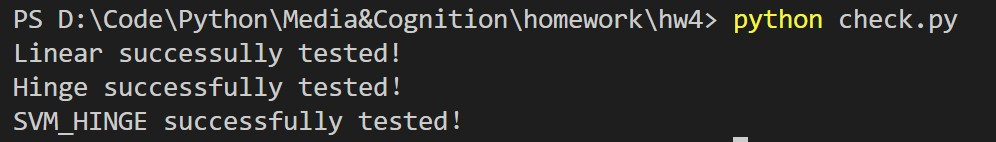
\includegraphics[width=12cm]{Fig_1.jpg}
    \caption{自动评判程序}
\end{figure}

\subsection{Hinge loss模拟SVM的训练及验证}
按要求补全代码,使用缺省参数训练,有以下结果:\\
测试集正确率:92.8\%\\

\subsection{可视化分类结果}
默认参数训练结果:(图2、图3、图4)\\
\begin{figure}
    \centering
    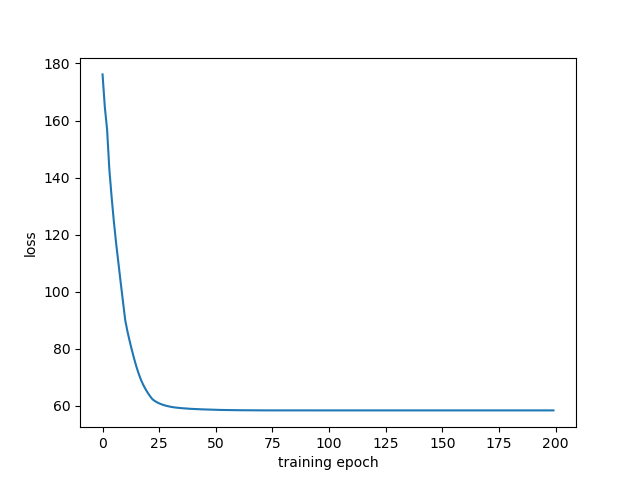
\includegraphics[width=12cm]{Fig_2.png}
    \caption{默认参数训练loss曲线}
\end{figure}
\begin{figure}
    \centering
    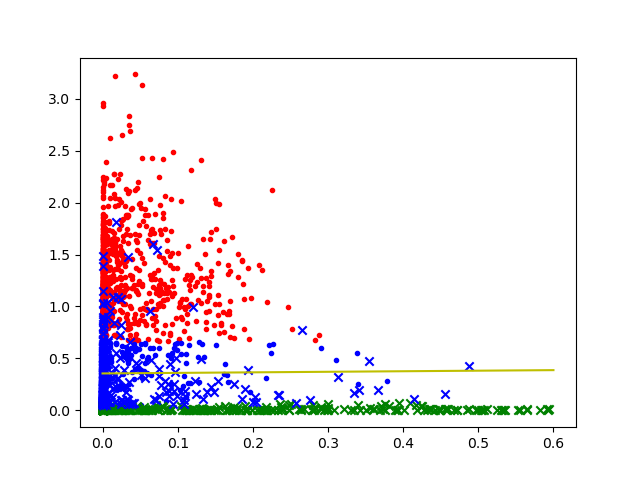
\includegraphics[width=12cm]{Fig_3.png}
    \caption{默认参数训练支持向量}
\end{figure}
\begin{figure}
    \centering
    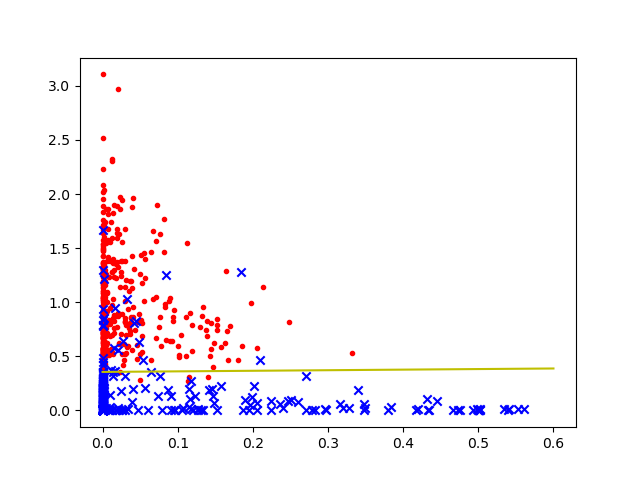
\includegraphics[width=12cm]{Fig_4.png}
    \caption{默认参数训练分类面}
\end{figure}

使用libsvm库进行分类:(图5、图6),结果如下:\\
nu = 0.266243 \\
obj = -58.385376, rho = 1.178906 \\
nSV = 641, nBSV = 638 \\
Total nSV = 641 \\
Accuracy = 92.75\% (742/800) (classification)\\
\begin{figure}
    \centering
    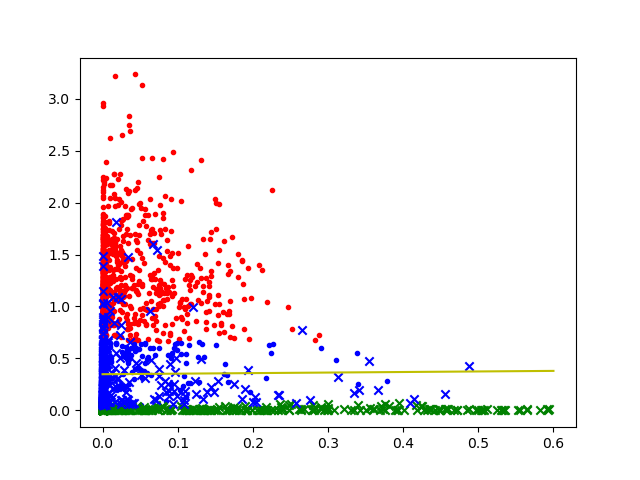
\includegraphics[width=12cm]{Fig_5.png}
    \caption{libsvm库支持向量}
\end{figure}
\begin{figure}
    \centering
    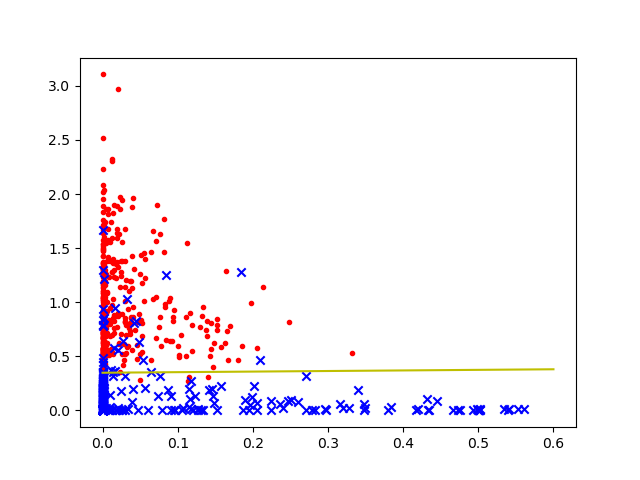
\includegraphics[width=12cm]{Fig_6.png}
    \caption{libsvm库分类面}
\end{figure}
比较两种方式的结果:训练出的模型准确率及分类界面都与libsvm库中相似,因此说明训练过程较为成功,未能分开的部分是由于训练集其自身原因有误差。

\subsection{调整正则化系数C}
取$ C=0.0001 $:\\
此时由于C较小,训练过程中loss均处于较低的值,验证集准确率始终为50\%左右,没有达到训练效果,完全欠拟合(图7)\\
\begin{figure}
    \centering
    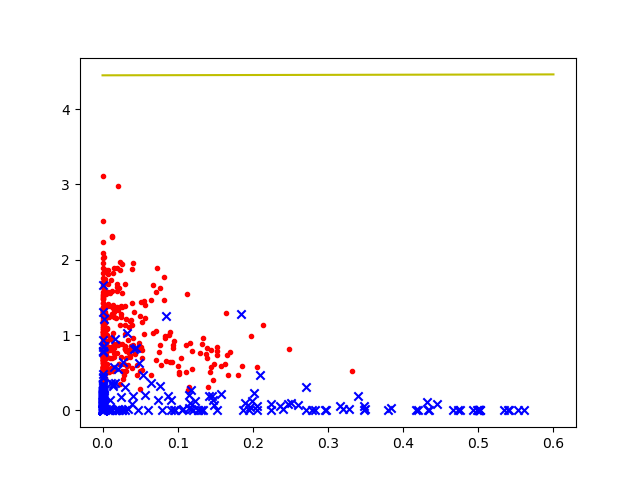
\includegraphics[width=12cm]{Fig_7.png}
    \caption{$ C = 0.0001 $训练分界面}
\end{figure}

取$ C = 0.001 $:\\
此时C仍较小,但训练过程中起到了一定的作用,验证集准确率达到68\%左右,仍为欠拟合(图8)\\
\begin{figure}
    \centering
    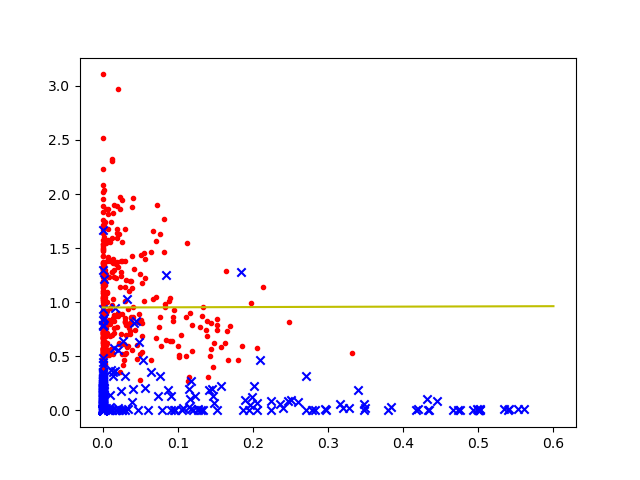
\includegraphics[width=12cm]{Fig_8.png}
    \caption{$ C = 0.001 $训练分界面}
\end{figure}

取$ C = 0.01 $:\\
此时C增大了一些,在训练过程中为模型提供了正则化,验证集准确率达到91\%左右,达到较好的分类效果(图9)\\
\begin{figure}
    \centering
    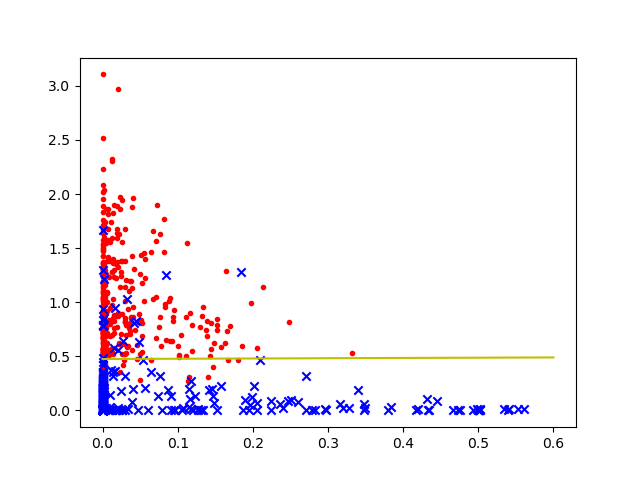
\includegraphics[width=12cm]{Fig_9.png}
    \caption{$ C = 0.01 $训练分界面}
\end{figure}

取$ C = 0.1 $:\\
此为默认参数训练,结果如前所述,分类效果较好(图4)\\

取$ C = 1 $:\\
此时C增大一些,仍能够提供较好的正则化效果,在验证集中正确率可达92\%(图10)\\
\begin{figure}
    \centering
    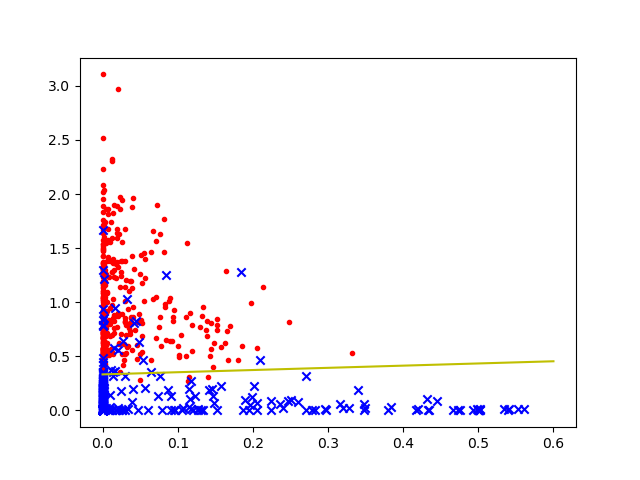
\includegraphics[width=12cm]{Fig_10.png}
    \caption{$ C = 1 $训练分界面}
\end{figure}

取$ C = 10 $:\\
此时C较大,仍能够提供较好的正则化效果,在验证集中正确率可达92\%(图10)\\
\begin{figure}
    \centering
    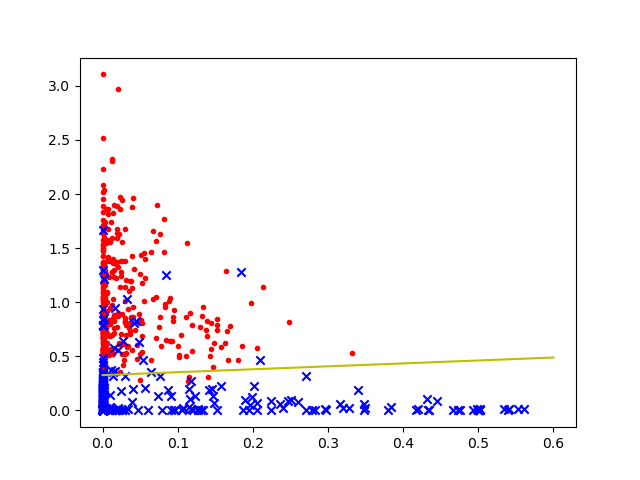
\includegraphics[width=12cm]{Fig_11.png}
    \caption{$ C = 10 $训练分界面}
\end{figure}

综上可以看出,C的选择在较小时会造成欠拟合,设置较大能够保证模型训练效果(这是由于此处模型为线性分类模型,并不复杂,对于复杂模型C过大可能会导致其它反作用)。

\end{document}



%%% Local Variables:
%%% mode: late\rvx
%%% TeX-master: t
%%% End:
